There are multiple technologies available to utilize in a solution. This chapter will contain information, descriptions and examinations of the considered technologies, as well as definitions used in the report.

Firstly, the controller units for the sensors will be described. These are necessary to process the information from the sensors and relay information between other nodes in the system.

Secondly, sensor devices are studied to be able to choose an adequate unit for the solution.

Thirdly, communication devices are examined to select an appropriate unit to use in the solution. 
\todo{Secondly, thirdly i forhold til det sidste?}

In the last part of the chapter, network topologies and communication protocols are examined to determine the best way of creating a network of nodes transmitting sensor data.

The chosen components, network type, and protocol can be found in Chapter \#\#. (Design chapter?)

\section{Platforms}
The suitable platforms for this project are examined in the following section. These platforms are capable of executing instructions as well as reading or writing to pins available on the board. These pins can be connect to components such as sensors and actuators.

\subsection{Arduino}\label{sec:arduino}
Arduino is an open source platform, which makes the software and hardware documentation available to the public. The name "Arduino" covers both the software platform and the range of hardware platforms with boards of different sizes, from the smaller Arduino Nano up to the Arduino Mega. One of the more popular Arduino boards is the Arduino Uno which is a medium sized board, often used by starters \cite{arduinouno}.

How the Arduino handles or reacts to input is implemented by the user and uploaded to the Arduino board by using the Arduino IDE.

\textbf{Arduino Uno}\\
One of the most common Arduino boards is the Uno, seen in figure \ref{fig:arduinouno}, which uses the ATmega328 microcontroller \cite{arduinouno}. It has 14 digital input/output pins, and 6 analog inputs for connecting different components. Considering specifications, which is shown in table \ref{tab:arduspecs}, the Uno is limited on its resources. Therefore it is needed to limit both program and data size, and also the amount of complex tasks.

\begin{figure}[h!]
\centering
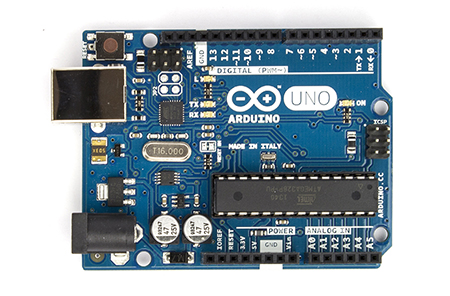
\includegraphics[width=0.5\textwidth]{chapters/analysis/figs/ArduinoUno.jpg}
\caption{The Arduino Uno board\cite{arduinointroduction}.}
\label{fig:arduinouno}
\end{figure}

\bgroup
\def\arraystretch{1.1}
\begin{table}[ht!]
\rowcolors{2}{gray!25}{gray!7}
%	\centering
	\begin{tabular}{p{15em} c c}
		Unit                        & Arduino Uno                                                                 & Arduino Mega                                                               \\ \hline
		Microcontroller             & ATmega328                                                                   & ATmega1280                                                                 \\
		Clock Speed                 & \multicolumn{2}{c}{16 MHz} \\
		Operating Voltage           & \multicolumn{2}{c}{5V}                                                                                                                                   \\
		Input Voltage (recommended) & \multicolumn{2}{c}{7-12V}                                                                                                                                \\
		Input Voltage (limits)      & \multicolumn{2}{c}{6-20V}                                                                                                                                \\
		DC Current per I/O Pin      & \multicolumn{2}{c}{40 mA}                                                                                                                                \\
		DC Current for 3.3V Pin     & \multicolumn{2}{c}{50 mA}                                                                                                                                \\
		Analog Input Pins           & 6                                                                           & 16                                                                         \\
		Digital I/O Pins            & \begin{tabular}[t]{@{}c@{}}14\\ (6 provide PWM output)\end{tabular}         & \begin{tabular}[t]{@{}c@{}}54\\ (15 provide PWM output)\end{tabular}       \\
		Flash Memory                & \begin{tabular}[t]{@{}c@{}}32 KB\\ (0.5 KB used by bootloader)\end{tabular} & \begin{tabular}[t]{@{}c@{}}128 KB\\ (4 KB used by bootloader)\end{tabular} \\
		SRAM                        & 2 KB                                                                        & 8 KB                                                                       \\
		EEPROM                      & 1 KB                                                                        & 4 KB                                                                       \\                
	\end{tabular}
	\caption{Arduino Uno and Mega specifications \cite{arduinouno}\cite{arduinomega}.}
\end{table}\label{tab:arduspecs}
\egroup


\textbf{Arduino Mega}\\
The Arduino Mega is a larger version of the Uno. The Mega has more memory and pins, which makes it better for handling larger programs and amounts of data, and also allows more components to be connected to the board. Since the clock speed is the same as the Uno, the Mega will not process data faster\cite{ardcomp}.

\begin{figure}[h!]
\centering
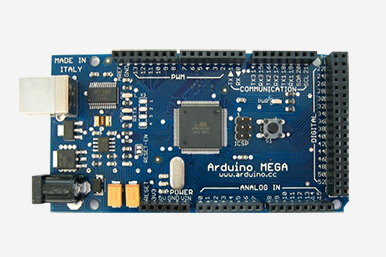
\includegraphics[width=0.6\textwidth]{chapters/analysis/figs/ArduinoMega.jpg}
\caption{The Arduino Mega board\cite{arduinomegaimg}.}
\label{fig:arduinomega}
\end{figure}

\subsection{Raspberry Pi}
Raspberry Pi is a series of single board computers. The Raspberry Pi series contains some powerful controllers compared to other pocket sized processing units.

The Raspberry Pi has a set of pins for connecting to external hardware. There are four different pin types available; two 5v power, two 3.3v power, five ground and 17 GPIO. In \figref{abPins} the placement of the pins is shown. 

The GPIO, or "general purpose input/output" pins can be used to either send or receive digital signals. Unlike the Arduinos it is stricly digital, as it does not have a build in analog to digital converter. If analog input processing is needed, this will have to be done externally.

\begin{figure}[H]
\centering
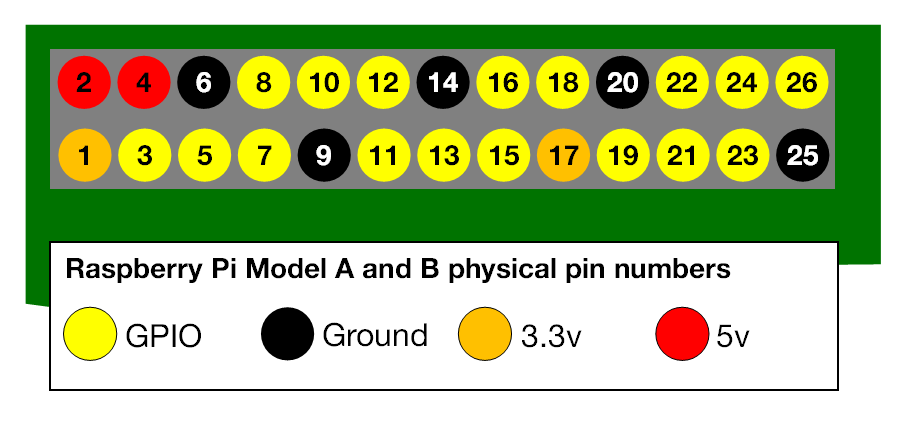
\includegraphics[width=0.6\textwidth]{chapters/analysis/figs/rpiABPins.png}
\caption{Raspberry Pi pins on model A and B.}
\label{fig:abPins}
\end{figure}

Because of the computing power and memory of a Raspberry Pi, a Linux OS is usually installed on the Raspberry Pi\cite{Arduino_linux}. A Raspberry Pi also has a GPU, video output, and USB port.

\textbf{Raspberry Pi B+}\\
In this subsection a Raspberry Pi B+ will be described as these were available to use in the project. The different models usually differs on CPU speed and memory.

The Raspberry Pi B+ specifications are shown in table \ref{tab:pibplusspec}. Futhermore the B+ also contains HDMI video output and Ethernet connectivity. A micro SD card is used as main storage a micro, which contains the OS.

\begin{figure}[H]
\centering
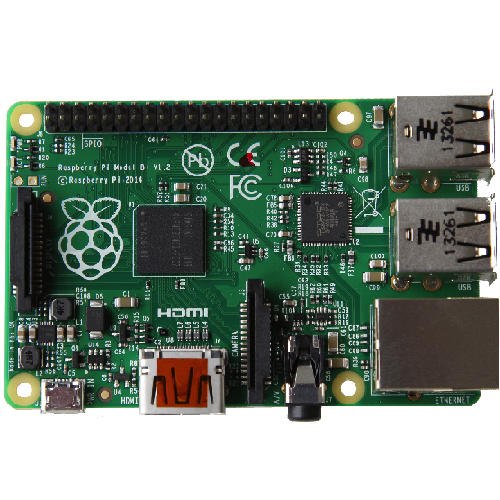
\includegraphics[width=0.6\textwidth]{chapters/analysis/figs/raspberry-pi-model-b-plus.png}
\caption{Raspberry Pi B+\cite{pibplus}.}
\label{fig:pibplus}
\end{figure}

\def\arraystretch{1.1}
\begin{table}[ht!]
\rowcolors{2}{gray!25}{gray!7}
\centering
\begin{tabular}{ l  l }
\hline
Microcontroller & Broadcom BCM2835\\
RAM & 512MB\\
Extended GPIO Pins & 40\\
USB Ports & 4\\
Clock Speed & 700 MHz\\
\hline
\end{tabular}
\caption{Specifications for Raspberry Pi B+\cite{pispecs}.}
\label{tab:pibplusspec}
\end{table}


\section{Sensors}
To gather relevant data from the real world, and handling this data in a digital domain, there has to be some sort of sensor that is capable of reading this data, and returning a value, either digitally or with an analog signal than can be read by a microprocessor.

\subsection{Moisture Sensor}
To obtain information about the moisture of the soil, a moisture sensor is needed. Simple moisture sensor are build as a pair of spikes inserted in the ground. Between them a current is being sent, and the resistance of the gound is checked. Based on this value the moisture can be calculated. %INSERTNAMEHERE\todo{find navnet -.-, og find documentation, er ebays beskrivelse gyldig?} .

\subsection{Soil pH Sensor}
To get information about the acidity or alkalinity of the soil, a pH is needed. These owever are both expensive and arguably unaccurate, so they will not be covered in depth. 

\subsection {Soil Compaction Sensor}
To get information about the compaction of the ground a sensor for measuring this can be helpful. However this is not data that changes as rapidly as moisture and pH. The slow datachanges and the pricepoint of sensors, which at time of writting is found from 200 usd and up, results in this sensor not being looked heavily into.


\section{Communication devices}
In the following section, different types of communication devices relevant to the project are examined. The goal is to determine which communication type and device is best suited\todo{no, to name/explain stuff, decision made in Design} for the solution.

\subsection{Bluetooth}
Bluetooth is a wireless technology standard designed to transfer data over short distances\todo{source}. Bluetooth is often used in phones and computers, and can be used to connect\todo{that's it? [she said]} devices, such as the ones to be designed as the solution. \todo{fix den her linje, er clueless.}

The number of devices that can be on a Bluetooth network is almost unlimited, and the the built-in interference reduction makes the technology usable for the product\todo{what prodct?} \cite{bluetoothbasics}.
Bluetooth devices have to be paired in order to exchange data, which makes it hard to create a hot pluggable network of devices\todo{why? motivate}. This, and the short maximum range of 100m\cite{bluetoothbasics}, makes it less\todo{than what?} adequate for this project, as golf courses are large and these devices will have to cover great distances.\todo{remember: no choices in this chapter}

\subsection{XBee}
XBee is a radio module by Digi. Multiple versions of the XBee modules exists, with differences in power usage, range, built-in/external antenna, and some with processors \cite{sparkfunXbeeGuide}.
XBees often use the ZigBee protocol. The ZigBee protocol is made for low-power devices, such as the product described in this report\cite{zigbee}.

\todo{JESUS, CHRIST! NO FREAKING "EASY" IN THE REPORT}
XBees are fast and predictable, making them a good choice for a project such as this. They can cooperate with the Arduino platform using the serial pins. There also exists special XBee shields made for Arduino.

XBees are unfortunately\todo{uheldigvis?} also quite expensive, which makes them unfit for this project. In later iterations\todo{a solution has no "later iterations". Further developement, fx?} of the solution \todo{vi bør diskuterre om det er produkt eller løsning?}\todo{bjørn synes det er en løsning på nogens problem, ikke et generelt produkt}  they could be used if longer ranges became a requirement or it had to interface with other devices using the ZigBee protocol or XBee modules.\todo{why is longer range requirement a counter argument for expensive?}

\subsection{RF24 Transceiver}\todo{aren't there several RF24s? we got the nRF24L01-something?}
The RF24 transceiver module is a radio module used for exchanging data between modules of the same type\todo{is this necessarily true? Can also communicate with other units using the same frequency?}. As with most of the XBee modules, the RF24 uses the 2.4GHz band, which is license-free in the whole world\todo{source}. It is well documented, and multiple libraries exists for using the device with Arduino\todo{well-documented: still no source?}.

The RF24 is cheaper than the XBees, and has shorter range and is potentially slower, depending on the communication protocol.

The full RF24 specifications can be seen in appendix \todo{add this.}

% The RF24 allows packets of up to 32 bytes, and is fast enough 


This section will contain descriptions of networks and network theory, and connect to the established use case.

A computer network is a collection of computers and devices connected so that they can share information and services \cite{mansfield2009computer}. The way these devices are interconnected is called topology. The communication structure the devices use to exchange information over a medium is called protocol, which will be described in another section.

In this section the term node is used for a device connected to the network, to avoid binding to a specific device type.

There are different types of network topologies, and here are some examples:
\begin{itemize}
	\item Ring
	\item Line
	\item Bus
	\item Tree
	\item Star
	\item Mesh
	\item Fully connected
\end{itemize}

These can be seen in figure xx, that will be put here somewhere. %The topologies considered for this use case are star, mesh, tree and ring networks. 

The star network has one main node that the other nodes are directly connected to. An example of a star topology network is wifi, typically with a wireless router to which other devices connect to gain network access. The wireless router will handle all the network communication and redirect the information to the correct device. A limitation of the star network is that all network devices must have a connection to the main node, and therefore be clustered within the reach of the main node coverage. 

A tree network also utilizes a main node, but the devices in the network do not necessarily connect directly to the main node, but rather connect to another node that relays to the main node. This can repeat over multiple levels, so that information is relayed through several nodes, before reaching the main node. The tree network has a fixed node structure, and the relay nodes will route the information towards the destination. 

Another topology is the mesh network. There are two kinds of mesh networks, the full-mesh and the partial-mesh networks. A full-mesh describes a network where all the nodes are interconnected, similar to a fully connected graph. A partial mesh is also a mesh network, but does not require all nodes to be connected, so that it's similar to a tree network with cycles. The mesh networks have the same limitation as a tree network, regarding the information transmission delay because the information transmits through up to several nodes. 

The best fitting network topology for the use case is a mesh network. It can transmit information through the network without limiting the connected devices to a certain distance from a main device, as with a star topology. It is also capable of multiple methods of distributing information. It does not rely on all nodes working at all times, as the network can reconfigure and find another path of information. This applies as long as there somehow exists another node that can relay the information towards the main node.

Move this paragraph?
There are multiple methods of communicating through a mesh network. Routing and flooding are two alternatives. Routing will transfer the information towards a destination node, whereas the flooding method will ask all nodes within reach to spread the information forwards, and this will repeat until all nodes has transmitted the information, and hence the destination node also has received the information.



%''\textit{An ad-hoc wireless network is a wireless network, comprised of mobile computing devices that use wireless transmission for communication, having no fixed infrastructure}'' - \cite{murthy2004ad}. 
\section{Communication protocols} \label{cha:comprot}
There are multiple methods for communicating in a network, and such a procedure is called a protocol \cite{protocol}. A protocol is a set of rules regarding, for example, the information format, procedures for sending and receiving, error discovery and handling, and it can be implemented in both hardware and software.

This section contains descriptions of multiple wireless network communication protocols that can be used in this project. These are considered and used as inspiration for the design and implementation of a protocl. First flooding protocols, followed by routing protocols.

There are many protocols and multiple groups of protocols, therein routing and flooding. 
Routing will transfer the information to the destination node through a determined route, whereas the flooding method will notify all nodes within reach to distribute the information forward, and this will repeat until all nodes has transmitted the information, and hence the destination node also has received the information.

%In networking, a protocol is a special set of rules and standards for how nodes(devices) would interacts with each other\cite{Protocol_difinition}.
%Well known protocols could be TCP/IP(Transmission Control Protocol/Internet Protocol), which affects every device connected to the internet.

Main node in this section is defined as the computer that handles that requests or sends the initial packet.
Packets are data sent though out the network. A packet can contain data to be delivered, or metadata to keep track of the packet, such as the sender ID of the packet.


\subsection{Flooding protocols}\label{cha:floodingSec}
Flooding in networks is a protocol used to deliver data throughout a network.
There are two kind of flooding: uncontrolled flooding and controlled flooding\cite{controlled_flooding}.

Uncontrolled flooding is the broadcasting of a packet, with a particular recipient, but without a particular route to reach the destination. Each node receiving the packet will repeat it to all of its neighbors, and they will repeat it again to theirs. This causes the packet to reach all nodes in the network, but it can cause communication loops. \cite{flooding}.

Controlled flooding is flooding protocols with filters or other measures to make it more reliable or efficient than the uncontrolled, hence avoiding cycles and broadcast \cite{controlled_flooding}.
Examples of such algorithms are Sequence Number Controlled Flooding (SNCF) and Reverse Path Flooding (RPF).
With SNCF, each node have its own address that is delivered with each data packet it transmits.
If a node receive a packet multiple times with the same unique id, the packet is discarded, so only one instance of the packet is transmitted.
In RPF, a node will forward a copy of a received packet, no matter the origin.
RPF expects that the original transmitted packet will be copied by the nodes in a path to the destination and eventual delivered\cite{RPF}.

Advantages of flooding, is that if there exists a route from the source to the destination, a packet will be delivered, and up to multiple times, depending on the implemented protocol.
Since some flooding algorithms utilizes every route in the network, it will also transfer packets through the shortest path\cite{flooding}.

Disadvantages can be that the bandwidth is wasted, since flooding is a very costly algorithm since it utilize every route.
Packets can be duplicated in the network, further increasing bandwidth load.
Duplicate packet may loop in the system forever, if no prevention is made \cite{flooding}.


\subsection{Time division multiple access}
Time division multiple access(TDMA) is an access protocol that divides a single channel into smaller time slots.
Each time slot is assigned to a single node, while every timeslot, are on the same channel.
Each timeslot is active a short period of time, allowing the assigned node to transmit, before the next node in the queue get time to transmit\cite{TDMA}.

%TDMA is, for example, used in the T1 telecommunication transmission system.\todo{relevance? what is T1?}
%Each T1 channels carry up to 24 voice telephone connections, where each connection covers 300 Hz to 3000Hz and is digitized at an 8-kHz rate, which is two times the highest frequency component needed to retain all the analog content.\todo{not protocol approach. very specific implementation example.}
\begin{figure}[!h]
	\centering
	\makebox[\textwidth][c]{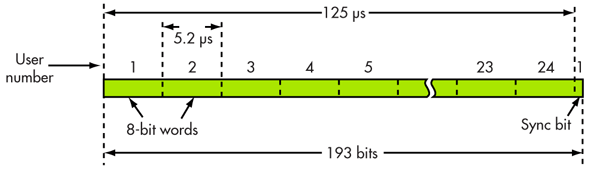
\includegraphics[width=1\textwidth]{figures/TDMA.png}}
	\caption{Illustration of the TDMA access method in the T1 protocol\cite{TDMA}.}
	\label{fig:TDMAfigure}
\end{figure}

In \figref{TDMAfigure} it is seen how the channel is split up into 24 smaller pieces. 
After the queue of timeslot there exists a bit, called the "Sync bit" as seen on the figure, that is used for synchronization.
Dividing the channel into smaller bites have little effect on the nodes transmission, because the shift between each time slot happens so fast.
This gives the illusion of each node communicating with no interruptions, even though each one is only assigned 1/24 of the total bandwidth on the channel.

TDMA can be used for any system that require several device to use the same channel, where interference can be a problem.
For example is radio transmitters a great fondness for causing interference, and that is in one of the areas TDMA can be used.\cite{interferance_protocols}



%\subsection{Radio Link Protocol}
%Radio Link protocol(RLP) is a automatic repeat request(ARQ)\footnote{An error-control method for data transmission that uses acknowledgements and timeouts} fragmentation protocol used over a wireless air interface.
%Most air interface protocols have a packet loss of up to 1\% which is intolerable when handling sensitive data.
%RLP detects losses in packets and with a retransmission tries to bring down the losses.
%The retransmission can bring the loss down to 0.1\% to 0.0001\%.
%This loss rate is more tolerable when handling sensitive and precise data.

%RPL cannot request a certain payload size from the air interface, the air interface scheduler instead determines the packet size, based on changing channel conditions constantly.
%Most of the other fragmentation protocols, such as 802.11b\footnote{An wireless networking specification} and IP, determine a payload of a certain size by the upper layers, and call upon the MAC.
%These protocols are not as flexible as RLP, and sometime fail transition during small fades in a wireless environment.\cite{MobileComm}

%RLP is used to make a more fail-safe environment for the transmitted data, and to ensure nothing is lost on the way.
%The Radio Link Protocol is typically used in cellular transmission.

\subsection{Dynamic Source Routing protocol}
The Dynamic Source Routing protocol (DSR) is a simple routing protocol designed specifically for use in wireless ad-hoc networks.
With DSR, the network is completely self-organizing and self-configuring, requiring no administration or existing network structure \cite{DSR}. 
As nodes can be added and removed as desired, the protocol automatically determine and maintain the routing of the packets through the network.
Since the number or sequence of nodes in a network, may change at any time, the topology may be quite rapidly changing.
DSR works on demand, allowing the routing of DSR to scales automatically affecting only nodes that is needed.
The protocol provides a highly responsive service to ensure successful delivery of data packets where node may be moving around, or other changes in the network occur\cite{DSR}. 

The DSR protocol is composed of two main mechanisms that allow the discovery and maintenance of the routes in the network.

- Route discovery is the mechanism by which a node S wishing to send a packet to a destination node D, obtains a route to D.
Route Discovery is used only when S attempts to send a packet to D and does not already know a route to D.

- Route maintenance is the mechanism by which node S is able to detect, while using a route to D, if the network topology has changed such that it can no longer use its route to D, which is known as a broken route.
When Route Maintenance indicates a route is broken, S can attempt to use any other route it happens to know to D, or it can invoke Route Discovery again to find a new route for subsequent packets to D.
Route Maintenance for this route is used only when S is actually sending packets to D.

DSR is a routing protocol where packets carries a header, an ordered list of nodes which is the route.
This explicit use of routing allows the sender to select and control the route for the packets it sends.
Routing allow for load balancing, since the sender can create different routes out though the network, avoiding high throughput through few nodes.
It is also a guarantee that the routes used are loop-free, since a generated route never use the same node twice.
By including this route in the header of each packet, other nodes forwarding or overhearing any of these packets can use this information for future use\cite{DSR}.
When a node overhear a packet with a route, the route is stored locally on the node.
The node can then use the route to forward messages, if its old route is unavailable.

\subsection{Ad-hoc On-Demand Distance Vector Routing}\label{cha:AOVD1}
Ad-hoc On-Demand Distance Vector(AODV) routing algorithm is a routing protocol designed for ad-hoc networks. 
It is an on-demand algorithm, meaning that it builds routes between nodes only as necessary by main nodes \cite{AOVD1}.

AODV is a network where only the nodes within reach of a newly added node is affected by the addition.
The transmission route in AODV is managed so that only nodes in the direct route are active.
The protocol can determine multiple routes between a main node and a destination, but only a single one is implemented, the route is not necessarily the shortest \cite{AOVD1}.

A disadvantage to AODV is that if a single route breaks, for example due to a defect node, it is not possible to know whether other routes exists.
A new route discovery in AODV is to be carried out before knowing if there exist a route.
If a link between nodes is broken, and it does not affect an ongoing transmission, no notification back to the main node occurs.

When a node is to forward a packet to a specified destination, it checks its routing table to determine if there currently exists a route to the destination.
The routing table is a table over every route though the node to any other, already discovered, destination.
If there already exist a route, the packet will be delivered to the next node in the route, repeating until it arrives at the correct location.
If there does not exist a route, the node will initiate a route discovery process \cite{AOVD1}.

A route discovery process in AODV begins with the main node creating a Route Request (RREQ) packet.
The packet contains the main node's unique ID and the destination node's unique ID.
The packet is then transmitted from the main node to it's neighbours.
The unique ID of each node is then appended to the packet, to ensure the same node is not transmitting more than once.
The destination ID is to ensure the nodes in the route knows when the destination node is reached.
A simple AODV network can be seen in \figref{AODVfigure}, where S and D represent the main node and destination. It is visualized how the route discovery is invoked using the RREQ packet.\cite{AOVD2}

\begin{figure}[!h]
	\centering
	\makebox[\textwidth][c]{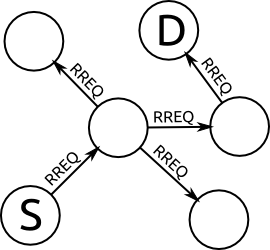
\includegraphics[width=0.4\textwidth]{figures/AODV.png}}
	\caption{Illustration of the AODV route discovery.}
	\label{fig:AODVfigure}
\end{figure}

\subsection{Better Approach To Mobile Ad-hoc Networking}
Better approach to mobile ad-hoc networking (B.A.T.M.A.N) is a routing protocol for ad-hoc mesh networks, based on AODV. 
B.A.T.M.A.N is said to solve some of the more typical problems with the classical routing protocols.
Some of the problems are, some networks are unstructured, can be based on an inherently unreliable medium and dynamically change their topology\cite{BATMAN}.

When using the B.A.T.M.A.N algorithm, the approach is to share the knowledge about the most reasonable path between nodes in a network to all of the participating nodes.
Each node in the network only account for the best path to all other nodes in the system.
This results in the need for a global knowledge about local topology changes becomes unnecessary.
In addition, B.A.T.M.A.N has an event-based, but timeless, flooding mechanism that prevents the occurrence of loops in the network.

Each node in the network transmits a broadcast message(called OGMs or originator messages in B.A.T.M.A.N) to inform every node within range about its existence.
The nodes within range, then re-broadcast the OGMs, to nodes within their range, about the existence of the original initiator of this message and so on.
This can result in the network being flooded with OGMs.
OGMs are small, the typical raw packet size is 52 byte including IP and UDP overhead\cite{BATMAN}.
OGMs contain at least the address of the originator, the address of the node transmitting the packet, and a sequence number.

OGMs that follow a path where the quality of wireless connection is poor will suffer from packet loss or delay on their way through the network.
Therefore OGMs that travel on good routes will propagate faster and be more reliable\cite{BATMAN}.

In order to tell if a OGM has been received once or more than once it contains a sequence number, given by the originator of the OGM.
Each node re-broadcasts each received OGM at most once and only those received from the neighbour which has been identified as the currently best next hop (best ranking neighbour) towards the original initiator of the OGM.

This way the OGMs are flooded selectively through the network and inform the receiving nodes about other node's existence. 
A node X will learn about the existence of a node Y in the distance by receiving it's OGMs, when OGMs of node Y are rebroadcasted by its neighbours.

The algorithm then selects this neighbour as the currently best next hop to the originator of the message and configures its routing table respectively \cite{BATMAN}.

\subsection{Protocol comparison}
Below is a comparison table with the protocol discuses in this chapter.
The four different protocols is compared in what route metric they are using, if they are loop free, support of load balancing, how reliable they are, and the estimated throughput.
This table is to create an overview of the protocols and to support a later choice of protocol of implementation.

\todo{actually compare the protocols?}

\begin{table}[!ht]
\caption{Protocol comparison.}
\label{my-label}
\makebox[\linewidth]{
\begin{tabular}{|l|c|c|c|c|c|c|}
\hline
            & Ad hoc & Route metrics                                                                     & \begin{tabular}[c]{@{}c@{}}Loop \\ Free\end{tabular} & \begin{tabular}[c]{@{}c@{}}Load \\ balancing\end{tabular} & Reliability & Throughput                                                                    \\ \hline%cline{1-1}
\rowcolor[HTML]{EFEFEF} 
TDMA\cite{TDMATable}        & Yes    & \begin{tabular}[c]{@{}c@{}}Routes ensuring\\  guaranteed bandwidth\end{tabular} & Yes                                                  & Yes                                                       & High        & \begin{tabular}[c]{@{}c@{}}Decreases as more \\ nodes are added\end{tabular} \\
DSR\cite{ProtocolTable}\cite{DSR}         & Yes    & Source routing                                                                   & Yes                                                  & No                                                        & High        & \begin{tabular}[c]{@{}c@{}}Decreases as more\\  nodes are added\end{tabular} \\
\rowcolor[HTML]{EFEFEF} 
AOVD\cite{ProtocolTable}        & Yes    & \begin{tabular}[c]{@{}c@{}}Fastest \&\\ shortest path\end{tabular}               & Yes                                                  & No                                                        & High        & \begin{tabular}[c]{@{}c@{}}Poor for more\\  than 20 nodes\end{tabular}       \\
B.A.T.M.A.N\cite{BATMAN} & Yes    & \begin{tabular}[c]{@{}c@{}}Fastest \&\\ shortest path\end{tabular}               & Yes                                                  & No                                                        & High        & \begin{tabular}[c]{@{}c@{}}Good - scales\\ well with more nodes\end{tabular} \\ \hline
\end{tabular}}
\end{table}

\iffalse %temporary removed
\subsection{Flooding as a routing algorithm}\label{cha:floodingSec}
Flooding in networks, is a routing algorithm used to deliver data out though a system.
There exists two kind of flooding, uncontrolled flooding and controlled flooding.
Uncontrolled flooding is a kind of "brute force", where every node, in a network, keeps sending the same packets indefinitely out to all its neighbours within range, creating what is known as a broadcast storm.
The packet will eventually the packet will reach its destination, without knowing when\cite{flooding}.

Controlled flooding is modified algorithms to make it reliable, some of algorithms are knows as Sequence Number Controlled Flooding(SNCF) and Reverse Path Flooding(RPF).
With SNCF each node have its own address that is delivered with each data packet it transmits.
If a node receive a packet twice or more with the same address, the packet is discarded, so only one instants of the packet is working its way though the network.
In RPF, the node will forward a copy of a received packet, no matter the origin.
RPF except that the original transmitted packet will be copied by the right nodes and eventually end at the destination\cite{RPF}.

Advantaged of flooding, is that if there exists a route from the main node to the destination, a packet will be delivered, and possible multiple times.
Since some flooding algorithms utilized every route in the network, it will also transfer packets though the shortest path\cite{flooding}.

Disadvantages can be that the bandwidth is wasted, since flooding is a very costly algorithm since it utilize every route.
Packets can be duplicated in the network, future increasing bandwidth load.
Duplicate packet may loop in the system forever, if no prevention is made\cite{flooding}.

\todo{flooding: take 2}
\fi
